\section{Discussion} 
\label{sec:Discussion}

% \subsection{Matched features}
% In this section, we discuss matched features to investigate prediction
% performance on cross-domain defect prediction in detail.
% 
% \begin{figure}[t]
% 	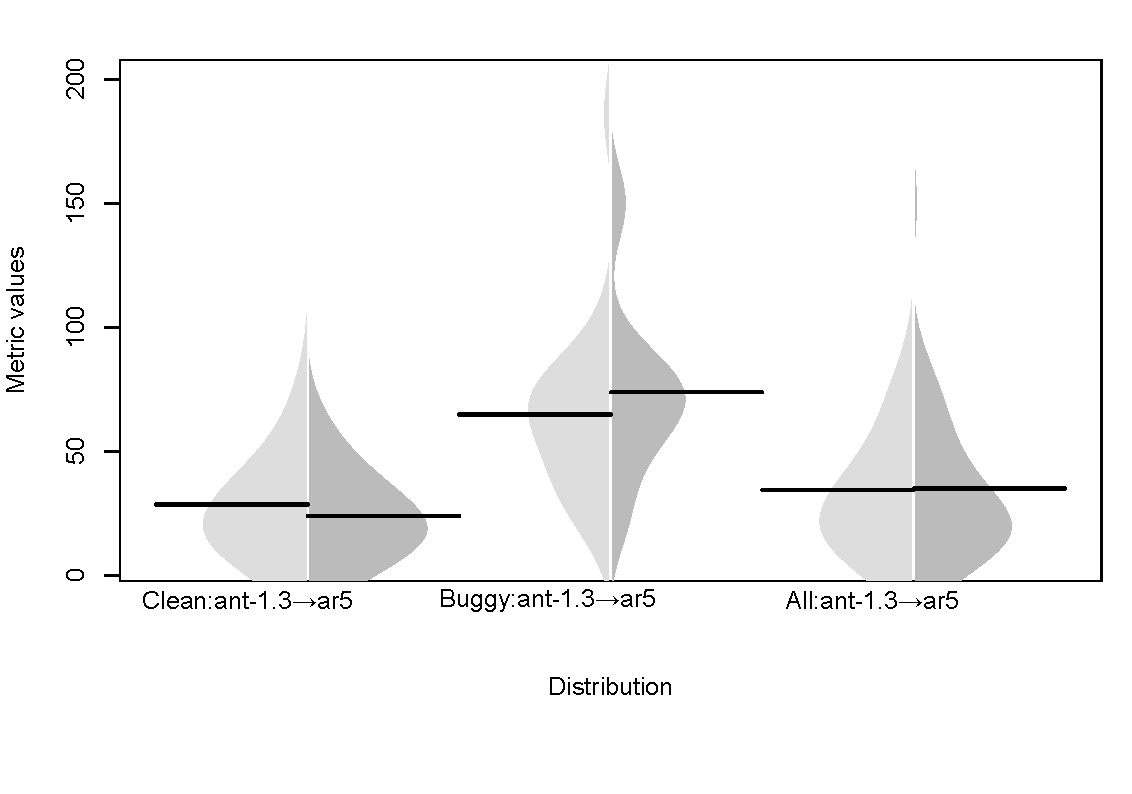
\includegraphics[width=\linewidth]{Figures/Result/best_dist.pdf}
% 	\caption{Feature value distribution of a matched feature from the
% 	prediction combination, ant-1.3$\Rightarrow$ar5, of AUC=0.938.}
% 	\label{fig:best_dist}
% \end{figure}
% 
% % A reason why ASAnalyzer can predict defects pretty well on cross-domain
% % settings is that most defect prediction metrics usually represent complexity of
% % source code and its change; it tends to be more buggy when the complexity is
% % higher.
% 
% In Figure~\ref{fig:best_dist}, we used beanplots~\cite{Beanplot08} to represent
% the feature value distribution of a matched feature in the prediction
% combination, ant-1.3$\Rightarrow$ar5, whose AUC is 0.938. The left side (light
% grey) of each beanplot shows distribution of buggy, clean, and all instances of
% source respectively, while the right side (dark grey) of each beanplot
% represents those of target. The horizontal black line represents an average
% value in each distribution. 
% 
% From Figure~\ref{fig:best_dist}, we can explain how ant-1.3$\Rightarrow$ar5 can
% have such a high AUC, 0.938. Suppose that a simple model predicts an instance as
% buggy when the feature value of the instance is more than 40 in case of
% Figure~\ref{fig:best_dist}. In both the source and target, approximately
% 70\% or more buggy and clean instances will be predicted correctly. In
% Figure~\ref{fig:best_dist}, the matched source and target features in
% ant-1.3$\Rightarrow$ar5 are the response for class (RFC: number of methods
% invoked by a class~\cite{Chidamber94}) and the number of unique operands
% (unique\_operands), respectively. The RFC and unique\_operands are not the same
% features. However, they have similar distribution as shown in
% Figure~\ref{fig:best_dist}. As we explained in Section~\ref{sec:Approach},
% typical defect prediction metrics (features) have a tendency that a higher
% complexity causes more buggy- proneness. The matched features
% follow this tendency very well so that the model using the matched features
% could achieve such a high AUC (0.938).
%but related; both features can be a factor contributing to how long and complex
% the source code is. In ar5, there is a more related feature such as comment\_loc. However, they are not actually matched since they have different distribution in terms of mean and standard deviation.

% \begin{figure}[t]
% 	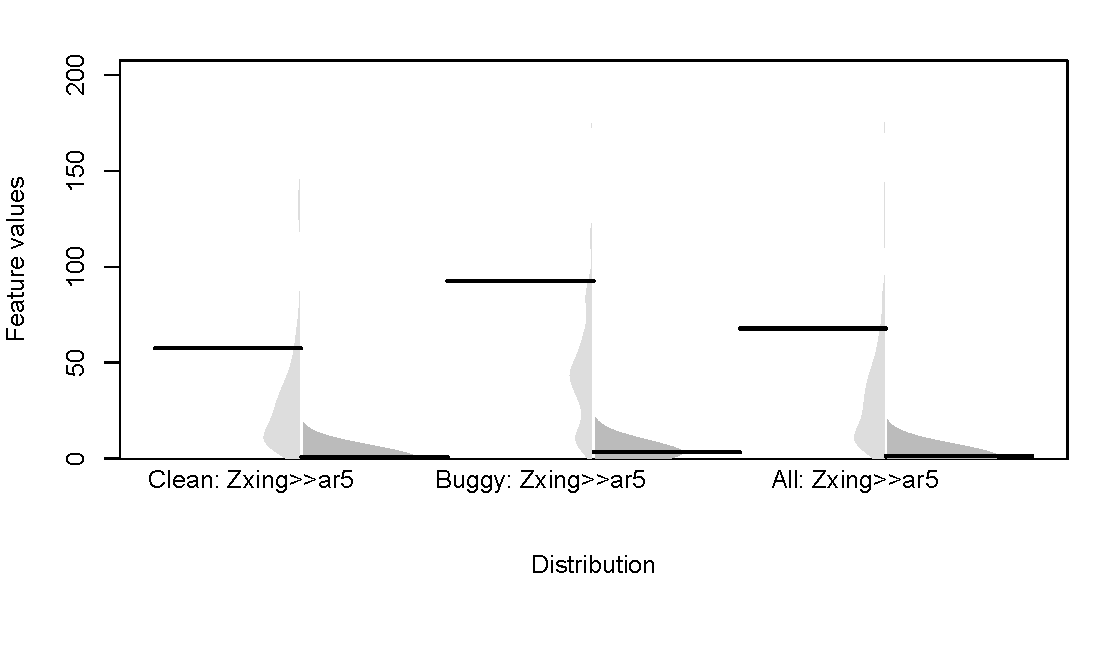
\includegraphics[width=\linewidth]{Figures/Result/beanplot_manual_matching.pdf}
% 	\caption{Feature value distribution of a manually matched feature (attribute)
% 	from the prediction combination, Zxing$\Rightarrow$ar5, of AUC=0.57.}
% 	\label{fig:manual_dist}
% \end{figure}
% 
% Each project
% may have different feature distributions even in projects with the same features
% since project characteristics can be made different by many other external
% environments such as the number of developers, product types, intended audiences, and so on.~\cite{Zimmermann09}.
% 
% Figure~\ref{fig:manual_dist} shows the feature value distribution of a
% manually matched feature of the prediction combination, Zxing$\Rightarrow$ar5, with AUC=0.57. The
% source and target features are CountLineCode and code-and-commend-loc
% respectively. Both features measure lines of code and comments, however their
% distributions are too different as seen in Figure~\ref{fig:manual_dist}. This
% is why cross-project prediction on projects with the same feature space is
% still a challenging issue~\cite{He12, Turhan09,Zimmermann09}. Thus, we tried to
% match features, which have similar distribution in a mechanical way to compare
% statistical parameters such as mean and standard deviation and observed
% many better prediction (Win) performance results as shown in
% Table~\ref{tab:win_results}.






\subsection{Practical Guidelines for HDP}

We proposed the HDP models to enable defect prediction on software projects
by using training datasets from other projects even with heterogeneous metric sets.
When we have training datasets in the same project or in other
projects with the same metric set, we can simply conduct
WPDP or CPDP using recently proposed CPDP techniques
respectively~\cite{Canfora13,Ma12,Nam13,Panichella14,Ryu14,Ryu15}.
However, in practice, it might be that no training datasets for
both WPDP and CPDP exist. In this case, we can apply the HDP approach.

In Section~\ref{sec:Result} and Table~\ref{tab:other_analyzers}, we confirm
that many target predictions in HDP by KSAnalyzer with the cutoff of 0.05
outperform or are comparable to those in WPDP and the HDP predictions show 100\% target coverage.
Since KSAnalyzer can match similar source and target metrics, we guide the use
of KSAnalyzer for HDP. In terms of the matching score cutoff threshold, there is a
trade-off between prediction performance and target coverage. Since a cutoff
of 0.05 that is the widely used level of statistical
significance~\cite{Corder09}, we can conduct HDP using KSAnalyzer with the
cutoff of 0.05. However, we observe some Loss results in our empirical study.
To minimize the percentage of Loss results, we can sacrifice the target coverage
by increasing the cutoff as Table~\ref{tab:other_analyzers} shows KSAnalyzer with
the cutoff of 0.90 led to 77.8\% Win results in feasible predictions against
WPDP.
By controlling a cutoff value, we may increase the target coverage.
For example, we can start from a higher cutoff value and decrease the cutoff until HDP is eligible.
This greedy approach might be helpful for practitioners who want to increase the target coverage when conducting HDP.
We remain validating this idea as a future work.

% However, we also observed Loss results and figured out filtering out Loss cases
% is quite challenging. When the metrics in defect datasets did not follow the
% common bug-prone tendency, our proposed HDP approach might not work well. We
% have a plan to address this challenging issue as future work.
% 
% Until addressing the issue about Loss cases, we can use KSAnalyzer with higher
% cutoffs. This option setting can mitigate Loss cases as KSAnalyzer with the
% cutoff of 0.90 achieved 100\% Wins in our experimental setting. However, the
% target coverage is only 21\%. To achive the 100\% target coverage, we might
% need more source datasets that have metrics matched with target metrics under
% KSAnalyzer with the cutoff of 0.90.

% \subsection{The number of matched features}
% \begin{table}[t]
% \small
% \centering
% \caption{The average number of matched features for each analyzer with
% cutoffs of 0.00, 0.05 and 0.90, and common features.}
% \label{tab:numFeatures}
% \begin{tabular}{|c|c|c|c||c|}
% \hline
% 
% % \multirow{2}{*}{{\bf Target}} &\multicolumn{3}{c||}{{\bf Cross by ASF}}
% % &\multicolumn{3}{c|}{{\bf Cross by manual}} \\ \cline{2-7}
% %  &Min & Max & Avg. &Min & Max & Avg. \\
% \multirow{2}{*}{{\bf Analyzer}}	& \multicolumn{3}{c||}{\specialcell{\bf{Average
% Number of}\\ {\bf Matched Features}}} &
% \multirow{2}{*}{\specialcell{\bf{Average number of}\\ \bf{Common Features}}} \\
% \cline{2-4} & {\bf 0.00} & {\bf 0.05} & {\bf 0.90} & \\
% \hline \hline
% 
% PAnalyzer			&7 &6 &1 & \multirow{4}{*}{5} \\ \cline{1-4}
% KSAnalyzer	&4 &2 &1 & \\ \cline{1-4}
% SCoAnalyzer			&7 &7 &6 & \\ \cline{1-4}
% PiAnalyzer			&7 &7 &6 & \\ \hline
% \end{tabular}
% \end{table}
% 
% Table~\ref{tab:numFeatures} shows the average number of matched
% features in prediction combinations between source and target datasets in each
% analyzer with cutoffs, 0.00, 0.05, and 0.9, and common features.
% 
% In KSAnalyzere with the cutoff of 0.00, the average number of matched features
% is four that is smaller than that (7) of other analyzers. The reason is that all
% matched features in some prediction combinations have matching scores of 0.00 so
% that these cross-predictions could not be conducted since there is no
% matched features whose matching scores are greater than 0.00 in the final set
% of matched features.
% For example, all matching scores in pc4$\Rightarrow$tomcat are 0.00 by
% KSAnalyzer so that this cross-prediction could not be conducted.
% 
% The average number of matched features in PAnalyzer and
% KSAnalyzer with the cutoff of 0.90 is one. The reason why the average
% number of matched features decreases is that poorly matched features with low
% matching scores automatically excluded according to the cutoff value.
% Many prediction combinations were not conducted because matched features whose
% matching scores are greater than 0.90 did not exist. Only 95 and 11 out of 600
% prediction combinations could be conducted in PAnalyzer and KSAnalyzer with the
% cutoff of 0.90 respectively.
% 
% However, the average number of matched features in ScoAnalyzer and PiAnalyzer
% seldom change. This means that the matching scores are very high in most matched
% features. Thus, using ScoAnalyzer and PiAnalyzer to match features between
% source and target datasets may not be helpful to judge whether matched features
% are similar or not.

\subsection{Threats to Validity}

%The selection of subjects used in our experiment can
%	be a threat. 
%Although we used 28 datasets for the experiment, 
%We used 28 datasets in our experiments for evaluating HDP models. Particularly for RQ1, this may lead to an issue about external validity since the 28 datasets may not be representative to conclude the results for RQ1. However, we tried to select various datasets used in papers published in top software engineering venues~\cite{DAmbros12,Lessmann08,Nam13,Peters12,Turhan09,Wu11}. In addition, we used datasets from both open-source (AEEEM~\cite{DAmbros12,Nam13}, ReLink~\cite{Wu11}, and MORPH~\cite{Peters12}) and proprietary projects (NASA~\cite{Lessmann08,Turhan09} and SOFTLAB~\cite{Turhan09}). For RQ2, we conducted Monte Carlo simulation for the generality of the RQ2 results. This can mitigate the issue of the external validity in our experiments.

We evaluated our HDP models in AUC.
	AUC is known as a good measure for comparing different prediction
	models~\cite{Giger12,Lessmann08,Rahman12,Song11}. However, validating
	prediction models in terms of both precision and recall is also required in
	practice. To fairly compare WPDP and HDP models in precision
	and recall, we need to identify a proper threshold of prediction probability.
	Identifying the proper threshold is a challenging issue and remains as
	future work.

For RQ1, we computed matching scores using all
	source and target instances for each prediction combination.
	With that matching scores, we tested prediction models on a test set from the two-fold cross validation because of the WPDP models as explained in Section~\ref{sec:expdesign}.
	To conduct WPDP with all instances of a project dataset as a test set, we need a training dataset from the previous releases of the same project. However, the training dataset is not
	available for our subjects. This may lead to an issue on construct validity since the matching score computations are not based on actual target instances used in the samples of the two-fold cross validation. To address this issue, we additionally conducted experiments with different sample sizes, i.e., 50, 100, 150, and 200 rather using all instances when computing matching scores for HDP in Section~\ref{sec:sizelimit}.

A recent study by Tantithamthavorn et al.~\cite{Tantithamthavorn16} pointed out model validation techniques may lead to different interpretation of defect prediction results. Although the n-fold cross validation is one of widely used model validation techniques~\cite{Klas2010,Nam13,Pinzger2008}, our experimental results based on the two-fold cross validation may be different from those using other validation techniques. This could be an issue in terms of construct validity as well.

Since we used the default options for machine learners in our experiments, the experimental results could be improved further when we use optimized options~\cite{Tantithamthavorn16icse,Fu2016}. Thus, our results may be affected by the other options tuning machine learners. We remain conducting experiments with the optimized options as a future work. 
%	about HDP against CPDP-CM and CPDP-IFS by testing a prediction model on a
%	test set using all instances of a target dataset in each prediction
%	combination.
%	In this setting, the median AUC of HDP was 0.723 and the median AUCs of the corresponding results in CPDP-CM and CPDP-IFS were 0.636 and 0.555
%	respectively.
%	These results are similar to those from the 50:50 random splits in
%	Section~\ref{sec:Result}. In other words, as long as the bug-prone tendency of matched metrics is consistent, HDP yields
%	promising results.
	

% In Section~\ref{sec:Result}, we found that cross-domain defect prediction from
% defect to defect datasets outperformed within-predictions with a higher
% chance; the percentages of Win+Tie were about 74\% and 82\% in the average
% F-measure and AUC, respectively. This result shows the possibility to improve
% defect prediction performance by using other defect datasets with different feature spaces.
% 
% \TODO{Analysis on co-occurrent features} To investigate how cross-domain defect
% prediction can build better prediction models, we took a closer look at the co-occurrent features identified by the
% co-occurrence analyzer.
% 
% \TODO{Analysis on SE and non-SE datasets}
% 
% \TODO{Summary of extensive and large scale results on different machine
% learning algorithms and co-occurrence analyzers with different cutoff values}
% Table~\ref{tab:win_results_on_diffrent_analyzers_ml_algs} represents the best win/tie/loss F-measure and AUC results on different analyzers and machine
% learning algorithms in our experimental settings. Results varies by analyzers
% and algorithms.
% Overall, PcoAnalyzer and Random forest lead to the best results comparing to other
% results. For example,...
% 
% \begin{table}
% \centering
% \caption{Best Win/Tie/Loss buggy F-measure and AUC results on different
% co-occurrent analyzers and machine learning (ML) algorithms.}
% \label{tab:win_results_on_diffrent_analyzers_ml_algs}
% %\setlength{\tabcolsep}{5pt}
% %\setlength{\extrarowheight}{1.5pt}
% \begin{tabular}{|@{ }c@{ }|@{ }c@{ }||@{ }c@{ }|@{ }c@{ }|@{ }c@{ }|@{ }c@{
% }||@{ }c@{ }|@{ }c@{ }|@{ }c@{ }|@{ }c@{ }|}
% \hline
% 	\multirow{2}{*}{\textbf{Analyzer}}
% 	&\multirow{2}{*}{\textbf{ML}}
% 	&\multicolumn{4}{c||}{\textbf{F-measure}}
% 	&\multicolumn{4}{c|}{\textbf{AUC}}
% 	\\ \cline{3-10}
% 	
% 	&
% 	&\textbf{cutoff}
% 	&\textbf{W}
% 	&\textbf{T}
% 	&\textbf{L}
% 	&\textbf{cutoff}
% 	&\textbf{W}
% 	&\textbf{T}
% 	&\textbf{L}
% 	\\ \hline \hline
% 	
% 	\multirow{7}{*}{AsAnalyzer}
% 	& J48
% 	&	0.65
% 	&	129 & 38 & 112
% 	&	0.65
% 	&	162 & 64 & 53
% 	\\ \cline{2-10}
% 	
% 	
% 	& RF
% 	&	0.80
% 	&	136 & 33 & 110
% 	&	0.85
% 	&	136 & 76 & 67
% 	\\  \cline{2-10}
% 	
% 	
% 	& NB
% 	&	0.80
% 	&	33 & 48 & 208
% 	&	0.90
% 	&	22 & 88 & 169
% 	\\  \cline{2-10}
% 	
% 	& BN
% 	&	0.75
% 	&	46 & 24 & 209
% 	&	0.70
% 	&	57 & 83 & 139
% 	\\  \cline{2-10}
% 	
% 	& LR
% 	&	0.70
% 	&	91 & 48 & 140
% 	&	0.80
% 	&	47 & 80 & 152
% 	\\  \cline{2-10}
% 	
% 	& MP
% 	&	0.75
% 	&	124 & 38 & 117
% 	&	0.65
% 	&	100 & 77 & 102
% 	\\  \cline{2-10}
% 	
% 	& SVM
% 	&	0.65
% 	&	143 & 28 & 108
% 	&	0.80
% 	&	122 & 63 & 94
% 	\\  \hline
% 	
% 	\multirow{7}{*}{TAnalyzer}
% 	& J48
% 	&	0.00
% 	&	131 & 44 & 104
% 	&	0.00
% 	&	164 & 64 & 51
% 	\\ \cline{2-10}
% 	
% 	
% 	& RF
% 	&	0.00
% 	&	123 & 46 & 110
% 	&	0.00
% 	&	132 & 80 & 67
% 	\\  \cline{2-10}
% 	
% 	
% 	& NB
% 	&	0.00
% 	&	37 & 39 & 203
% 	&	0.95
% 	&	16 & 65 & 165
% 	\\  \cline{2-10}
% 	
% 	& BN
% 	&	0.95
% 	&	30 & 12 & 204
% 	&	0.00
% 	&	54 & 85 & 140
% 	\\  \cline{2-10}
% 	
% 	& LR
% 	&	0.00
% 	&	82 & 52 & 145
% 	&	0.95
% 	&	34 & 60 & 152
% 	\\  \cline{2-10}
% 	
% 	& MP
% 	&	0.00
% 	&	120 & 36 & 123
% 	&	0.35
% 	&	65 & 86 & 128
% 	\\  \cline{2-10}
% 	
% 	& SVM
% 	&	0.00
% 	&	152 & 27 & 100
% 	&	0.00
% 	&	122 & 61 & 96
% 	\\  \hline
% 	
% 	\multirow{7}{*}{PcoAnalyzer}
% 	& J48
% 	&	0.75
% 	&	138 & 40 & 101
% 	&	\bf{0.80}
% 	&	\bf{167} & \bf{70} & \bf{42}
% 	\\ \cline{2-10}
% 	
% 	
% 	& \bf{RF}
% 	&	\bf{0.80}
% 	&	\bf{133} & \bf{49} & \bf{97}
% 	&	0.35
% 	&	142 & 82 & 55
% 	\\  \cline{2-10}
% 	
% 	
% 	& NB
% 	&	0.95
% 	&	39 & 35 & 205
% 	&	0.90
% 	&	19 & 101 & 159
% 	\\  \cline{2-10}
% 	
% 	& BN
% 	&	0.95
% 	&	52 & 32 & 195
% 	&	0.85
% 	&	51 & 96 & 132
% 	\\  \cline{2-10}
% 	
% 	& LR
% 	&	0.45
% 	&	90 & 52 & 137
% 	&	0.90
% 	&	49 & 75 & 155
% 	\\  \cline{2-10}
% 	
% 	& MP
% 	&	0.00
% 	&	122 & 43 & 144
% 	&	0.80
% 	&	90 & 85 & 104
% 	\\  \cline{2-10}
% 	
% 	& SVM
% 	&	0.90
% 	&	142 & 36 & 101
% 	&	0.15
% 	&	128 & 59 & 92
% 	\\  \hline
% 	
% % 	\multirow{6}{*}{ScoAnalyzer}
% % 	& J48
% % 	&	0.x
% % 	&	18 & 0 & 8
% % 	&	0.x
% % 	&	18 & 0 & 8
% % 	\\ \cline{2-10}
% % 	
% % 	
% % 	& RF
% % 	&	0.x
% % 	&	18 & 0 & 8
% % 	&	0.x
% % 	&	18 & 0 & 8
% % 	\\  \cline{2-10}
% % 	
% % 	
% % 	& NB
% % 	&	0.x
% % 	&	18 & 0 & 8
% % 	&	0.x
% % 	&	18 & 0 & 8
% % 	\\  \cline{2-10}
% % 	
% % 	& BN
% % 	&	0.x
% % 	&	18 & 0 & 8
% % 	&	0.x
% % 	&	18 & 0 & 8
% % 	\\  \cline{2-10}
% % 	
% % 	& LR
% % 	&	0.x
% % 	&	18 & 0 & 8
% % 	&	0.x
% % 	&	18 & 0 & 8
% % 	\\  \cline{2-10}
% % 	
% % 	
% % 	& SVM
% % 	&	0.x
% % 	&	18 & 0 & 8
% % 	&	0.x
% % 	&	18 & 0 & 8
% % 	\\  \hline
% 	
% 	
% 	\multirow{7}{*}{PiAnalyzer}
% 	& J48
% 	&	0.95
% 	&	132 & 35 & 112
% 	&	0.95
% 	&	159 & 65 & 55
% 	\\ \cline{2-10}
% 	
% 	
% 	& RF
% 	&	0.95
% 	&	126 & 33 & 120
% 	&	0.95
% 	&	139 & 70 & 70
% 	\\  \cline{2-10}
% 	
% 	
% 	& NB
% 	&	0.95
% 	&	34 & 30 & 215
% 	&	0.95
% 	&	17 & 88 & 174
% 	\\  \cline{2-10}
% 	
% 	& BN
% 	&	0.95
% 	&	48 & 27 & 204
% 	&	0.95
% 	&	55 & 86 & 138
% 	\\  \cline{2-10}
% 	
% 	& LR
% 	&	0.95
% 	&	88 & 45 & 146
% 	&	0.95
% 	&	38 & 88 & 153
% 	\\  \cline{2-10}
% 	
% 	& MP
% 	&	0.90
% 	&	112 & 32 & 135
% 	&	0.95
% 	&	77 & 83 & 119
% 	\\  \cline{2-10}
% 	
% 	& SVM
% 	&	0.95
% 	&	133 & 31 & 115
% 	&	0.95
% 	&	115 & 59 & 105
% 	\\  \hline
% 
% \end{tabular}
% \end{table}


